\section{Descrição da metodologia}
\subsection{O Semáforo}
\setlength{\parindent}{2cm}
O semárofo teve como partida a idealização da máquina de estados de alto nível representada na figura abaixo: 
\begin{figure}
\caption{FSM do semáforo}
\centering
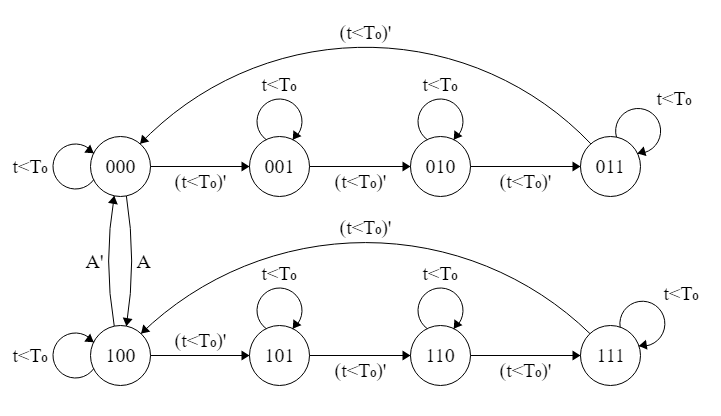
\includegraphics[width=0.75\columnwidth]{fsmsemaforo.png}
\end{figure}
Onde as saídas dos estados dependem de um comparador t < T\textsubscript{0} que, por sua vez, depende de uma "memória" que armazena diferentes T\textsubscript{0} para atender aos diferentes tipos de temporização dos semáforos. A entrada "A" presente na RTL, é necessária devido à mudança para a temporização que faz os semáforos só piscarem amarelo. A implementação dela também é necessária já que as saidas dos estados "100" ao "111" não são análogas às saídas do resto dos estados.

A partir disso, idealizou-se um componente Datapath que é composto de um divisor de frequência, um contador (para contar os segundos), e um comparador (que irá informar ao controlador quando t $\geq$ T\textsubscript{0}, fazendo os estados avançarem).
\begin{figure}
\caption{Datapath do semáforo}
\centering
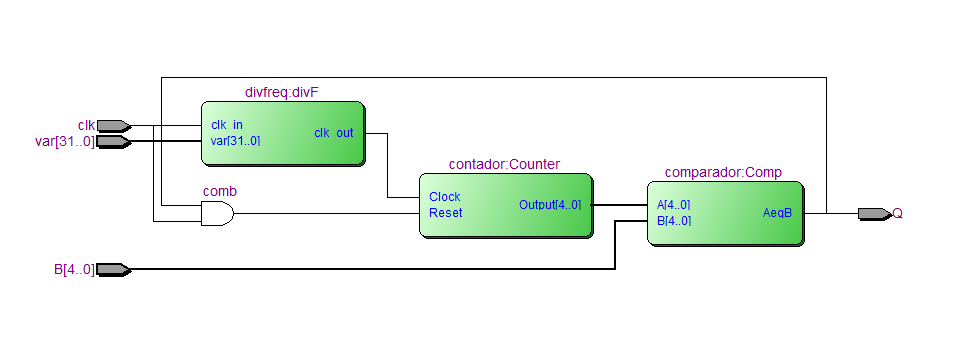
\includegraphics[width=0.75\columnwidth]{datapath.png}
\end{figure}

Com isso foi feito a Tabela verdade contendo os estados e saídas correspondentes:
\begin{figure}
\caption{Tabela Verdade do semáforo}
\centering
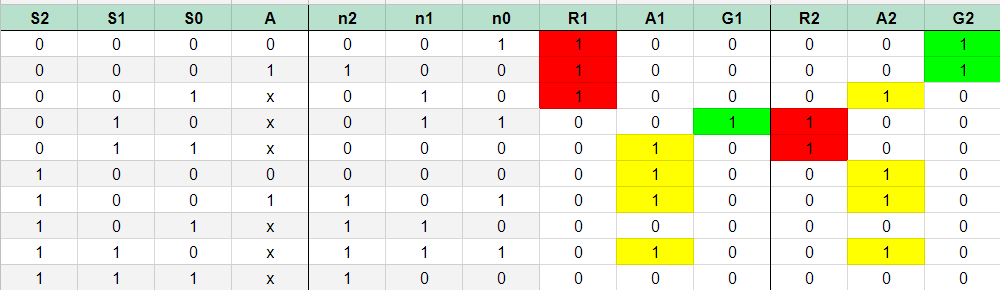
\includegraphics[width=0.75\columnwidth]{tv_semaforo.png}
\end{figure}

Outro aspecto dessa máquina de estados foi a implementação de um MUX que seleciona dentro de si a temporização de cada estado. O funcionamento dele está descrito na Table~\ref{tab01}.
\begin{table}[]
\caption{Mux de seleção de tempo}
\label{tab01}
\begin{tabular}{| c | c | c | c | c |}
\hline
Switches/Estados & 00 & 01 & 10 & 11  \\ \hline
00  & 30 & 3 & 10 & 3 \\ 
01  & 20 & 3 & 20 & 3 \\ 
10  & 1  & 1 & 1  & 1 \\ 
11  & -  & - & -  & - \\ \hline
\end{tabular}
\end{table}
Assim, esse MUX precisa de 4 entradas, duas dos Switches e duas de estado. Ou seja os bits mais significantes serão as entradas sw\textsubscript{1} e sw\textsubscript{0} e os menos significantes serão os bits menos significantes das entradas do estado atual da FSM, que chamaremos de s\textsubscript{1} e s\textsubscript{0}, que também serão saídas do controlador.

Juntando todas os componentes, finalizamos a entidade semáforo que ficou composta dessa maneira e obteve os seguintes resultados:
\begin{figure}
\caption{Circuito do Semáforo}
\centering
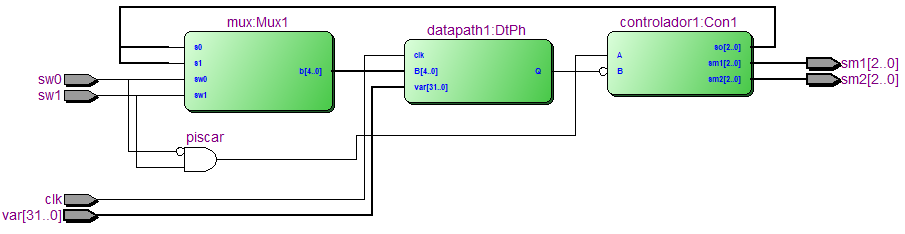
\includegraphics[width=0.75\columnwidth]{semaforo1.png}
\end{figure}

\begin{figure}
\caption{Waveform do Semáforo para os Modos 00 e 01}
\centering
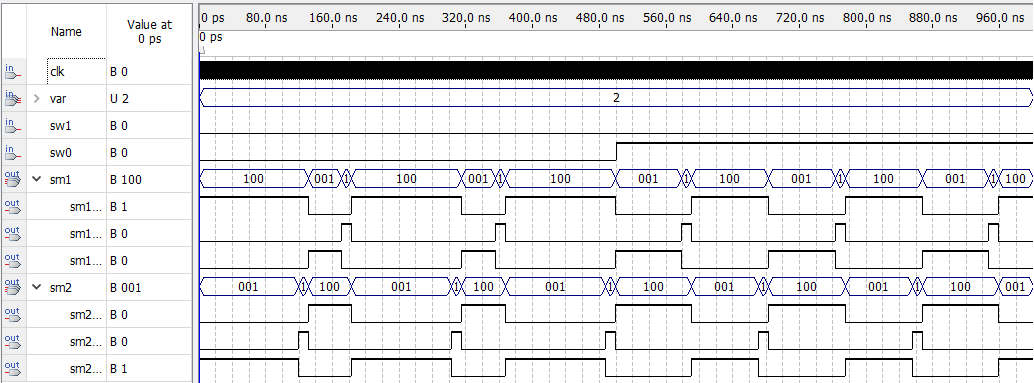
\includegraphics[width=0.99\columnwidth]{waveformsemaforo.png}
\end{figure}

\begin{figure}
\caption{Waveform do Semáforo para o Modo 10}
\centering
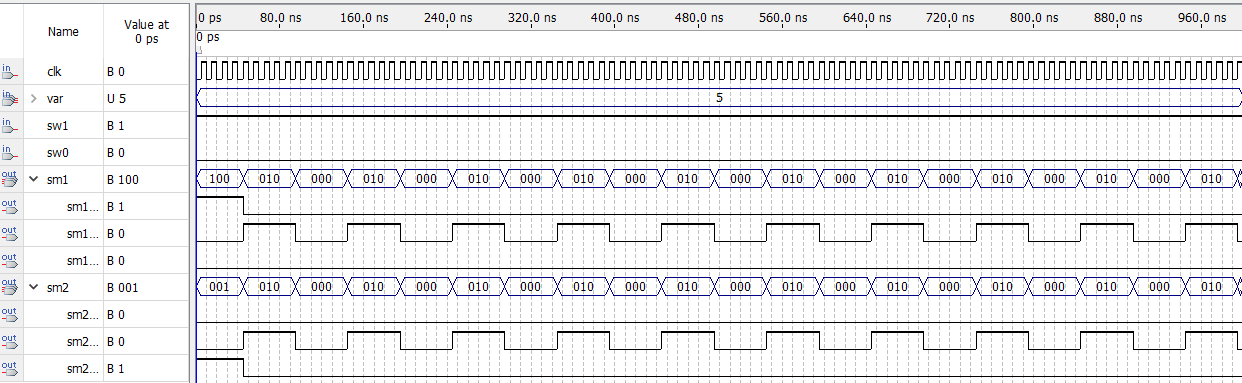
\includegraphics[width=0.99\columnwidth]{waveformpisca.png}
\end{figure}
Obs.: A entrada "var" é um inteiro que serve para o divisor de frequência, ela é definida quando se escolher o pino da FPGA que irá servir de clock. Para fins demonstrativos, dei valores baixos a essa variável, visto que a simulação de clock também é baixa.

\subsection{Radar de velocidade}
\setlength{\parindent}{2cm}
O radar foi idealizado, primeiramente com o seguinte diagrama RTL:
\begin{figure}
\caption{Diagrama RTL do Radar}
\centering
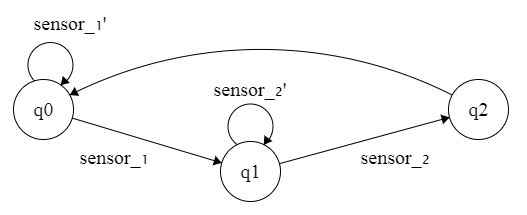
\includegraphics[width=0.75\columnwidth]{0.png}
\end{figure}

Porém, o projeto do radar foi mais simplificado, como os sensores estão separados em 30m e a velocidade máxima permitida é de 36km/h ou 10m/s, o carro precisa passar pelos dois sensores num intervalo de no mínimo 3 segundos. Precisavamos, então, implementar um contador juntamente de um comparador aliados à um divisor de freqruência. Assim, o nosso radar segue o seguinte modelo:
\begin{figure}
\caption{Modelo dos componentes do Radar}
\centering
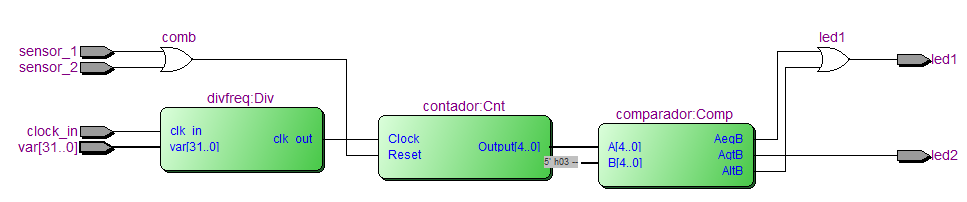
\includegraphics[width=0.99\columnwidth]{radar.png}
\end{figure}
Obs.: Esse modelo mudou com a adição da lógica que determina quando as luzes acendem ou apagam.

Com isso, percebemos que o sinal mandado dependeria também de qual botão foi apertado. Para tanto, foram criados sinais auxiliares que permitiram que as luzes de "acima da velocidade" ou "na velocidade permitida" fossem acesas somente após o carro passar pelo segundo sensor e desligadas assim que o próximo carro passar pelo primeiro. Por fim foi testado o radar e obtivemos o seguinte Waveform:
\begin{figure}
\caption{Waveform do Radar}
\centering
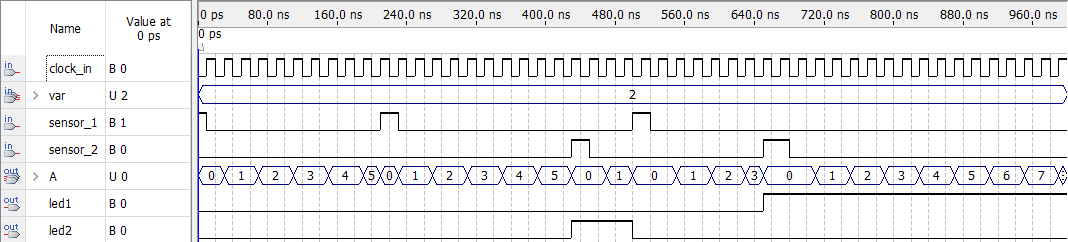
\includegraphics[width=0.99\columnwidth]{waveformradar.png}
\end{figure}
Obs.: O led\textsubscript{1} representa o sinal de velocidade permitida, e o led\textsubscript{2} representa o sinal de acima da velocidade permitida. Além disso a variável "A" foi adicionada para melhor visualização da contagem, porém não está presente no arquivo final.

\section{Conclusão}
\setlength{\parindent}{2cm}

Por fim, juntamos ambos as entidades "semaforo" e "radar" na implementação de um novo arquivo que conseguisse ser usado no FPGA para ambas funcionalidades. Com esse trabalho conseguimos aprofundar nossos conhcimentos nos assuntos abordados além de ampliar nossa base em VHDL, linguagem tão importate para nosso período acadêmico e vidas profissionais.
Os códigos fontes utilizados nesse trabalho estão disponíveis neste \href{https://github.com/angelomarcelino/circuitos-digitais/tree/master/Mobilidade_Urbana}{link}.